\documentclass[12pt]{article}
\usepackage[danish]{babel}
\usepackage[utf8]{inputenc} % Æ,Ø,å, æ ø,å på pc
\usepackage{amsthm,amssymb,amsmath,dsfont,mathrsfs,nicefrac}
\usepackage[pdftex]{graphicx}
\usepackage{epstopdf}
 % Matematiske pakker

\begin{document}


Man kan nu begynde at anvende de ligninger der er blevet udledt i de tidligere afsnit, på en cylinder.
\\
Der er givet en cylinders parameterfrenstilling:
\\
$r(\theta):=(cos(\theta),sin(\theta),z)$
\\
En geodætisk kurve henover denne cylinder kunne se således ud:
\\
$r(\theta):=(cos(\theta),sin(\theta),z(\theta))$
\\
Afstanden hen over cylinderen er givet ved Lagrangefunktionen, hvor S er et udtryk for længden
\\
$S = \sqrt{(\frac{d}{d\theta}(cos(\theta))^2+\frac{d}{d\theta}(sin(\theta))^2+\frac{d}{d\theta}(z(\theta))^2}d\theta$
\\
Simplificerer vi dette en smule får vi:
\begin{equation*}
S=\int_{\theta_a}^{\theta_b}\sqrt{(1+\dot{z}(z(\theta))^2}
\end{equation*}
\\
Hertil kan vi definerer funktionen der beskriver den differenterede længde.
\begin{equation*}
S=\sqrt{(1+(z(\theta))^2}
\end{equation*}
Skal S være så lille som muligt skal f dertil opfylder Euler-Lagrange differentialligning
\begin{equation}
\frac{\partial f}{\partial z}-\frac{d f}{d \theta} \frac{d f}{d\dot{z}}=0
\end{equation}
Da $\frac{\partial f}{\partial z}$ bliver Euler-lagrange ligning da:

\begin{equation}
\int_{\theta_a}^{\theta_b}\frac{d}{d\theta}\frac{\dot{z}\theta}{\sqrt{(1+\dot{z}(z(\theta))^2}d\theta}
\end{equation}
Differeteres der i forhold til theta fås der
\begin{equation}
\int_{\theta_a}^{\theta_b}\frac{\dot{\dot{z}}\theta}{\sqrt{(1+\\dot{\dot{z}(z(\theta))^2}d\theta}}
\end{equation}
For at denne skal give 0 skal tælleren have formen:
\begin{equation}
k\cdot \theta+C = z(\theta)
\end{equation}
k er et udtryk for hældning og C er bare en konstant.

Dette betyder at funktionen der forbinder 2 punkter på en cylinder er en ret linje hvilket jo også giver mening.
\\
\\
Vi kan nu opstille to ligninger til undersøgelse af hvilken effekt det vil have at ændre de forskellige parametre.

Første ligning
\begin{equation}
k\cdot \theta_a + C = z(\theta_a)
\end{equation}
Anden ligning
\begin{equation}
k\cdot \theta_b + C = z(\theta_b)
\end{equation}
hvor det gælder at
\begin{equation}
\begin{gathered}
z(\theta_a)=Z_a \\
z(\theta_b)=Z_b\\
\theta_a,\theta_b,\in[0;2\pi[ \\
\theta_a < \theta_b
\end{gathered}
\end{equation}
Hældningen for en ret linje mellem 2 punkter kan udtrykkes ved $\frac{\delta z}{\delta \theta}$

\begin{equation}
k=(\frac{z_a-z_b}{\theta_a-\theta_b})
\end{equation}
Vi kan hertil se hvad det betyder at $Z_a$ $\neq$
$Z_b$ sætte Za til 3 og Zb til 5 og vi sætter $\theta_a$ til $\frac{1}{2} \pi$ og $\theta_b$ til $\pi$

jeg indsætte mine værdier i første ligning
\begin{equation}
\frac{3-5}{\frac{1}{2}\pi-\pi}\frac{1}{2} \pi + C = 3
\end{equation}
Vi finder C
\begin{equation}
C = -2+3
\end{equation}
\begin{equation}
C = 1
\end{equation}
Her ses den geodætiske kurve plottet på en cylinder
\begin{figure}
\center
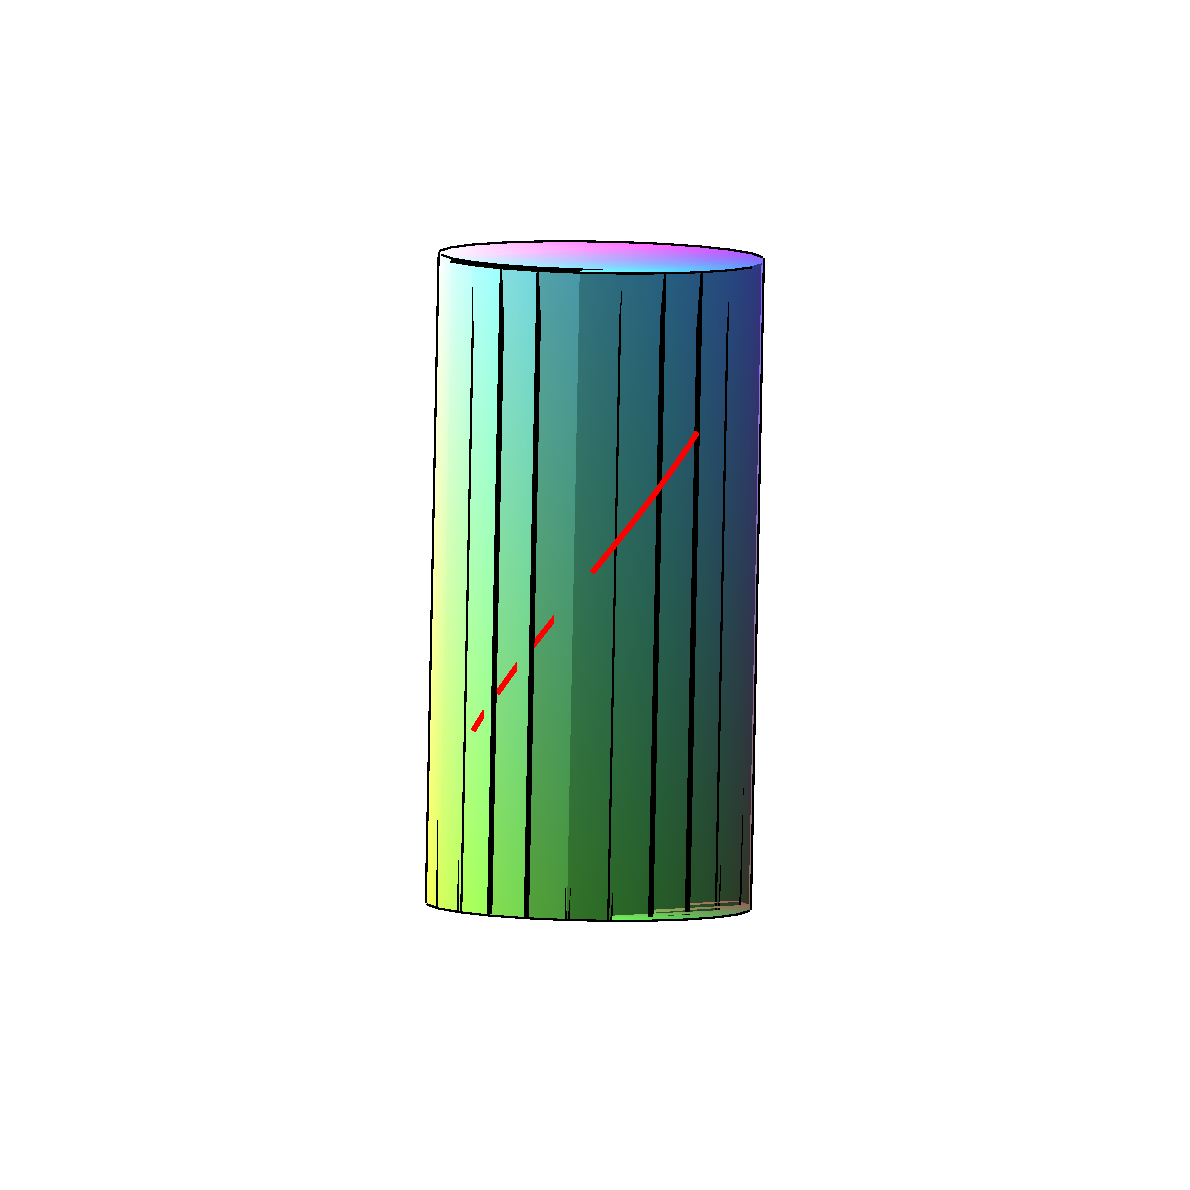
\includegraphics[scale=0.4]{pictures/Opg8_Fig1.eps}
\caption{lol hurr durr+}
\end{figure}


\end{document}